\documentclass[12pt]{article} % The document class with options

\usepackage[margin=1in]{geometry}
\usepackage[utf8]{inputenc} 
\geometry{a4paper}
\usepackage{newtxtext,newtxmath}
\usepackage[T1]{fontenc}
\usepackage{amsmath}
\usepackage{amsfonts}
\usepackage{microtype}
\usepackage{graphicx}
\usepackage{listings} % For formatting and highlighting code
\usepackage{color}    % For colors in code highlighting

% Define colors for syntax highlighting
\usepackage{color}
\definecolor{dkgreen}{rgb}{0,0.6,0}
\definecolor{gray}{rgb}{0.5,0.5,0.5}
\definecolor{mauve}{rgb}{0.58,0,0.82}

% Code listing style named "mystyle"
\lstset{frame=tb,
  language=Python,
  aboveskip=3mm,
  belowskip=3mm,
  showstringspaces=false,
  columns=flexible,
  basicstyle={\small\ttfamily},
  numbers=none,
  numberstyle=\tiny\color{gray},
  keywordstyle=\color{blue},
  commentstyle=\color{dkgreen},
  stringstyle=\color{mauve},
  breaklines=true,
  breakatwhitespace=true,
  tabsize=3
}
% chktex-file 3
% chktex-file 8
% chktex-file 10
% chktex-file 17
% chktex-file 18
% chktex-file 36
% chktex-file 44

\begin{document}
\setlength{\parskip}{1em} 
\setlength{\parindent}{0pt}
\newcommand{\vect}[1]{\mathbf{#1}}

\begin{titlepage}  % This starts a title page environment
    \centering    % Center everything on the page

    %--- Add space at the top of the page ---
    \vspace*{2cm}
    
    %--- Title ---
    \normalsize \textbf{MECH 503 Final Exam} \\

  
    \vspace{2cm}  % Space between the title and the author name
    
    %--- Author ---
    \normalsize by\\
    \vspace{1cm}
    \normalsize Jincong Li \\ 
    \vspace{1cm}
    \normalsize M.Eng, The University of British Columbia, 2024
    \vspace{11cm}  % Space between the author and the date
    
    %--- Date ---
    \normalsize \today

    \vfill  % Push the following content to the bottom of the page
    %--- Bottom part of the page ---
    © Jincong Li, 2024
\end{titlepage}
\tableofcontents
\newpage
\section{Question 1}
\begin{align*}
    BC_1 &= \sigma_{xy}(x,y=\pm \frac{h}{2}) = 0\\
    BC_2 &= \sigma_{y}(x,y=\frac{h}{2}) = 0\\
    BC_3 &= \sigma_{y}(x,y=\frac{-h}{2}) = -q\\
    BC_4 &= \int_{\frac{-h}{2}}^{\frac{h}{2}} \sigma_x(x=\pm L,y) = 0 \\
    BC_5 &= \int_{\frac{-h}{2}}^{\frac{h}{2}} \sigma_x(x=\pm L,y)y = 0 \\
    BC_6 &= \int_{\frac{-h}{2}}^{\frac{h}{2}} \sigma_{xy}(x=\pm L,y) = \pm Lq \\
\end{align*}
One could observe the boundary conditions are satisfied in classical and weak sense. For the normal stress in x-direction:
\[ \sigma_x(x=\pm L,y) = \pm \frac{q y \left(3 h^{2} - 20 y^{2}\right)}{5 h^{3}} \] which is symmetric about the y-axis, thus, the moment is balanced.
\begin{figure}[ht]
    \centering
    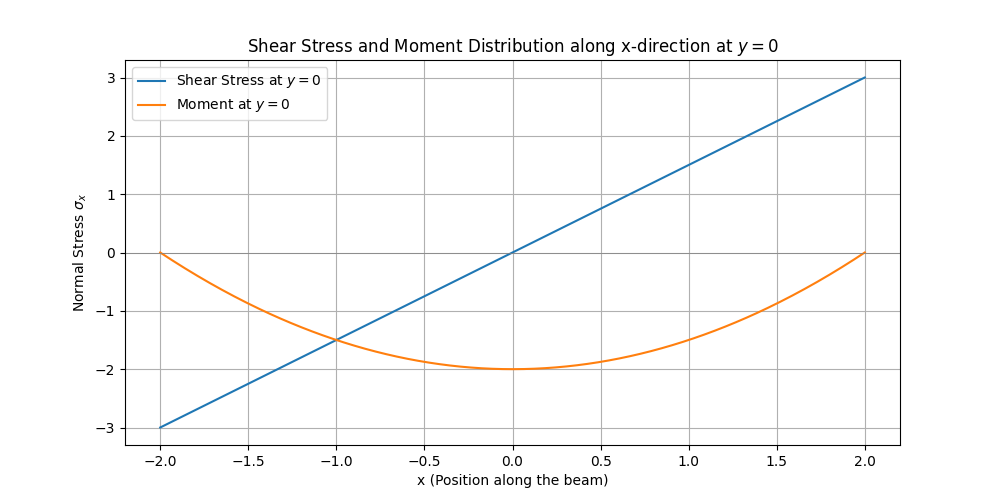
\includegraphics[width=1\textwidth]{Q1.png}
    \caption{Shear Stress and Moment Distribution along x-direction at $y=0$}
\end{figure}
The distribution of shear stress and moment is shown in figure 1, which agrees with the theory.

The Python code is provided in the Appendix file.

\section{Question 2}
\subsection*{Part 1}
\begin{align*}
    \sigma_{\theta\theta}(r=a) &= 0\\
    \sigma_{r\theta}(r=a) &= 0\\
\end{align*}
\subsection*{Part 2}
\begin{align*}
    \sigma_{rr}(\frac{r}{a}=\infty ) &= \sigma_{0} \sin^{2}{\left(\theta \right)}\\
    \sigma_{r\theta}(\frac{r}{a}=\infty ) &= - \frac{\sigma_{0} \sin{\left(2 \theta \right)}}{2}\\
    \sigma_{\theta\theta}(\frac{r}{a}=\infty ) &= \sigma_{0} \sin^{2}{\left(\theta \right)}\\
\end{align*}
\subsection*{Part 3}
\begin{align*}
    \sigma_{xx}(\frac{r}{a}=\infty ) &= - \sigma_{0} \sin^{2}{\left(\theta \right)} \cos{\left(2 \theta \right)}\\
    \sigma_{yy}(\frac{r}{a}=\infty ) &= - \frac{\sigma_{0} \sin{\left(4 \theta \right)}}{4}\\
    \sigma_{xy}(\frac{r}{a}=\infty ) &= - \sigma_{0} \sin^{2}{\left(\theta \right)} \cos{\left(2 \theta \right)}\\
\end{align*}
\newpage
\subsection*{Part 4}
\begin{figure}[ht]
    \centering
    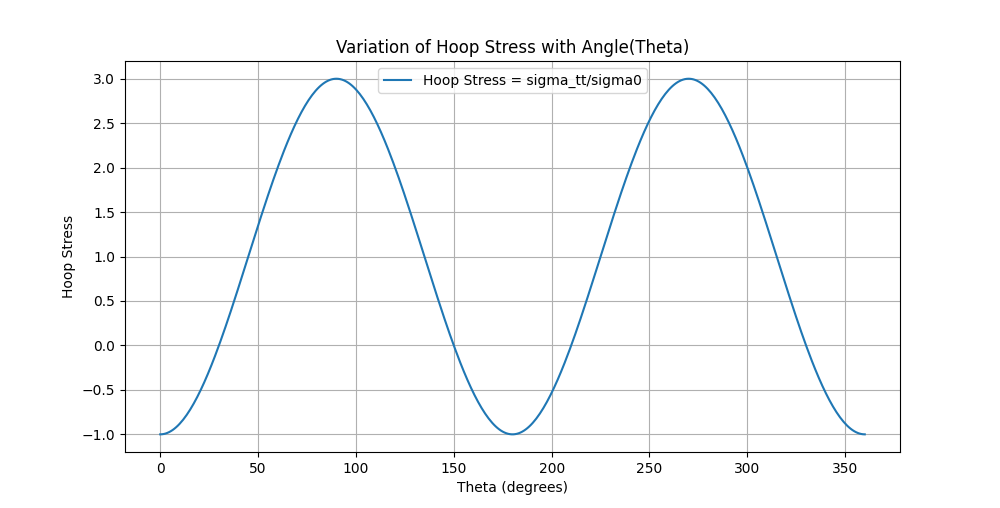
\includegraphics[width=1\textwidth]{Hoop Stress.png}
    \caption{Hoop Stress vs. Angle($\theta$)}
\end{figure}
The maximum value of hoop stress is 3, which occurs at $\theta$ = 90.0 degrees.
\subsection{Part 5}
\begin{figure}[ht]
    \centering
    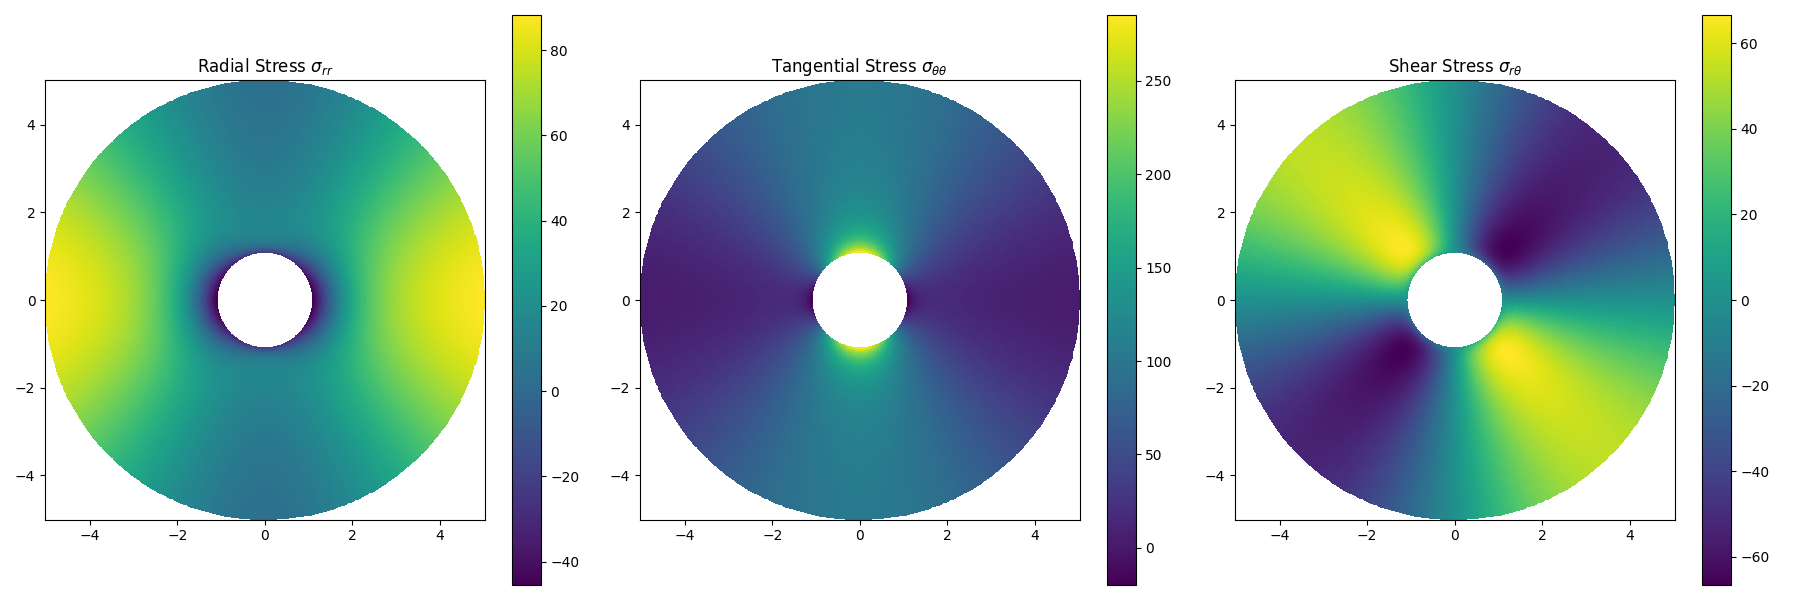
\includegraphics[width=1\textwidth]{Q2.png}
    \caption{Stress Distribution around the Hole}
\end{figure}

\section{Question 3}
\clearpage
\section{Question 4}
This question in coded in Python entirely, thus, for detail information, please refer to the code provided in Appendix file.
And also note that the computation process is modified according to the MATLAB code posted on Canvas.
\begin{figure}[ht]
    \centering
    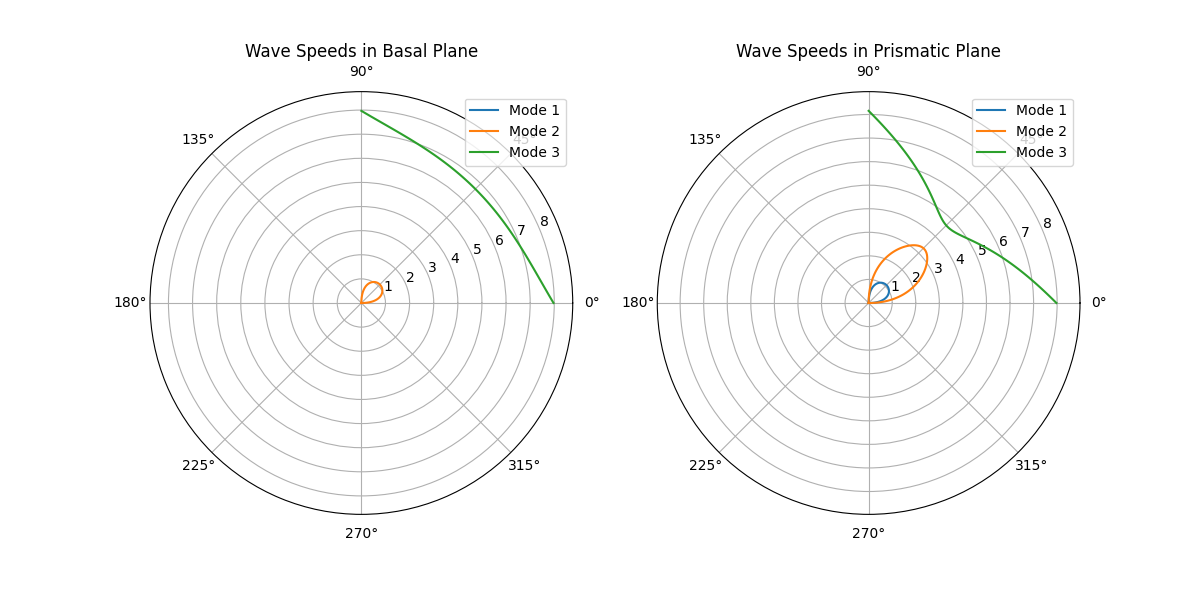
\includegraphics[width=1\textwidth]{Q4.png}
    \caption{Wave Speed Distribution in Polar Plot}
\end{figure}

\section{Question 5}
\section{Question 6}

\subsection*{Q3}
\subsection*{Q4}
\subsection*{Q5}
\subsection*{Q6}
\end{document}